\documentclass[./main]{subfiles}

\begin{document}
  \chapter{Algorithmes probabilistes.}

  Dans ce chapitre, on s'intéresse aux algorithmes probabilistes et les classes de complexité correspondantes.
  Le modèle de calcul sera les \textit{machines de Turing probabilistes}, qui ressemblent aux machines de Turing non-déterministes, mais pas exactement. Plus précisément, on aura deux fonction de transitions $\delta_0$ et $\delta_1$ et, à chaque étape, on applique $\delta_0$ (ou $\delta_1$) avec probabilité $1 / 2$.
  De plus, tous ces choix sont indépendants.

  \begin{rmk}
    Les machines de Turing déterministes sont des cas particuliers car il suffit de poser $\delta_0 := \delta =: \delta_1$, en notant $\delta$ la fonction de transition de la machine de Turing déterministe.
  \end{rmk}

  \begin{defn}
    La \textit{probabilité d'accepter} $w \in \Sigma^\star$ est
    \[
    \sum_{
      \begin{array}{c}
        \text{$b$ chemin de calcul}\\
        \text{acceptant sur l'entrée $w$}
      \end{array}
    } \Pr[b]
    ,\] 
    où, en notant $k$ la longueur du chemin,\footnote{Dans ce cas, c'est le nombre de tirages au sort.}
    \[
      \Pr[b] := \frac{1}{2^k}
    .\] 
  \end{defn}

  \begin{defn}
    Pour $0 \le \varepsilon < 1/2$, une machine probabiliste \textit{reconnait} un langage $A$ avec probabilité d'erreur $\varepsilon$ si
    \begin{enumerate}
      \item si $w \in A$ alors $\Pr[\text{$w$ est accepté}] \ge 1 - \varepsilon$ ;
      \item si $w \not\in A$ alors $\Pr[\text{$w$ est rejeté}] \ge 1 - \varepsilon$.
    \end{enumerate}
  \end{defn}

  On considère ensuite les machines probabilistes qui fonctionnent en temps polynomial en $|w|$.
  La machine s'arrêtera donc en un temps polynomial \textit{peu importe} les choix probabilistes.

  \begin{defn}
    On définit la classe $\intro*\bpp$\footnote{Pour \textit{Bounded Propability Polynomial}} comme la classe des langages qui peuvent être reconnus par des machines probabilistes qui fonctionnent en temps polynomial avec probabilité d'erreur~$1 / 3$.
  \end{defn}

  De manière analogue à la classe $\np$, on a une caractérisation par certificats pour $\bpp$.

  \begin{prop}
    Un langage $A$ est dans $\bpp$ si, et seulement si, il existe un polynôme $p$ et un problème auxiliaire $B \in \p$ tel que
    \begin{enumerate}
      \item si $x \in A$ alors $\Pr_{y \in \{\texttt{0},\texttt{1}\}^{p(|x|)}}[\code{x,y} \in B] \ge \frac{2}{3}$ ;
      \item si $x \not\in A$ alors $\Pr_{y \in \{\texttt{0},\texttt{1}\}^{p(|x|)}}[\code{x,y} \not\in B] \ge \frac{2}{3}$.
    \end{enumerate}
    Le choix de $y \in \{\texttt{0}, \texttt{1}\}^{p(|x|)}$ se fait avec la distribution uniforme.
    \qed
  \end{prop}
  
  Le choix de $\varepsilon = 1/3$ dans la définition de $\bpp$ peut sembler arbitraire mais, mais ça n'a pas d'importance comme le montre le lemme ci-dessous.

  \begin{lem}[d'amplification]
    Soit $0 \le \varepsilon < 1/2$.
    Supposons qu'un langage $A \subseteq \Sigma^\star$ est reconnu avec probabilité d'erreur $\varepsilon$ par une machine de Turing probabiliste polynomiale $M_1$.
    Pour tout polynôme $p(n)$, alors $A$ peut être reconnu par une machine probabiliste polynomiale $M_2$ avec probabilité d'erreur $2^{-p(n)}$ sur toute entrée de taille~$n$.
  \end{lem}
  \begin{prv}
    L'algorithme de $M_2$ est de la forme suivante.

    \begin{algorithmic}[1]
      \State Effectuer $2k$ calculs de $M_1$ sur l'entrée $x \in \Sigma^n$ \label{alg:amplificiation-l1}
      \If{$M_1$ accepte pour une majorité (stricte) de calculs}
      \State \textbf{Accepter}
      \Else
      \State \textbf{Rejeter}
      \EndIf
    \end{algorithmic}

    Il nous reste à déterminer la valeur de $k$ telle que 
    \[
      \Pr[\text{$M_2$ fasse une erreur sur l'entrée $x$}] \le \frac{1}{2^{p(n)}}
    .\]

    Pour $x$ donné, soit $S \in \{\texttt{0},\texttt{1}\}^{2k}$ la suite des résultats obtenus à la ligne~\ref{alg:amplificiation-l1}.
    Notons $c$ le nombre de résultats corrects et $w$ le nombre de résultats incorrects (on a donc $c + w = 2k$).
    On dit que $S$ est "\textit{mauvaise}" si $c \le w$ (autrement dit $w \ge k$).

    On a 
    \[
      \Pr[\text{$M_2$ fasse une erreur sur l'entrée $x$}] \le \sum_{S \text{ mauvaise}} \Pr[S]
    .\]
    On majore (grossièrement) le nombre de mauvaises suites $S$ par le nombre total de suites, \textit{i.e.}\ $2^{2k}$.
    En fixant une mauvaise suite $S \in \{\texttt{0},\texttt{1}\}^{2k}$, on a 
    \[
      \Pr[S] =
      \varepsilon(x)^w \cdot (1 - \varepsilon)^c = 
      \varepsilon(x)^k \cdot (1 - \varepsilon)^k \cdot \left( \frac{\varepsilon(x)}{1 - \varepsilon(x)} \right)^{w - k}
    ,\]
    en notant $\varepsilon(x)$ la probabilité que $M_1$ fasse une erreur sur l'entrée $x$ (on a donc $\varepsilon(x) \le \varepsilon$).
    Comme $w \ge k$ (car $S$ supposée mauvaise), on a 
    \[
    \left(\frac{\varepsilon(x)}{1 - \varepsilon(x)}\right)^{w-k} < 1
    .\]
    On en déduit $\Pr[S] \le \big(\varepsilon(x) (1 - \varepsilon(x))\big)^k$, d'où
    \begin{align*}
      \Pr[\text{$M_2$ fasse une erreur sur l'entrée $x$}] &{}\le \big(4 \varepsilon(x) (1-  \varepsilon(x))\big)^k\\
       &{}\le \big(4 \varepsilon (1-  \varepsilon)\big)^k
    .\end{align*}

    Il suffit ainsi d'avoir $[4 \varepsilon (1-\varepsilon)]^k \le 2^{-p(n)}$, autrement dit,
    \[
      k \ge \frac{p(n)}{-\log_2 [4 \varepsilon (1 - \varepsilon)]}
    .\]
  \end{prv}

  \begin{figure}
    \centering
    \begin{tikzpicture}
    \begin{axis}[
        domain=0:1,
        axis lines = left,
        xlabel={$z$},
        ylabel={$4z(1-z)$},
        ymin=0, ymax=1.15,
      ]
    \addplot[color=deepgreen, samples=100, thick]{4 * x * (1 - x)};
    \addplot +[mark=none,color=deepgreen,thick,dashed] coordinates {(0.5, 0) (0.5, 1)};
    \node[fill=white] (a) at (axis cs:0.5,0.3) {$1/2$};
    \addplot +[mark=none,color=deepgreen,thick,dashed] coordinates {(0.2, 0) (0.2, 0.64)};
    \node[fill=white] (c) at (axis cs:0.2,0.3) {$\varepsilon(x)$};
    \addplot +[mark=none,color=deepgreen,thick,dashed] coordinates {(0.35, 0) (0.35, 0.91)};
    \node[fill=white] (b) at (axis cs:0.35,0.3) {$\varepsilon$};
    \path (a) to node[midway] {$<$} (b);
    \path (b) to node[midway] {$\le$} (c);
    \end{axis}
    \end{tikzpicture}
    \caption{Graphe de $z \mapsto 4 z (1-z)$}
  \end{figure}

  \begin{prop}
    On a $\bpp \subseteq \pspace$.
  \end{prop}
  \begin{prv}
    On énumère tous les chemins de calcul possible, et on accepte si une majorité de ces chemins accepte.
  \end{prv}

  \begin{thm}
    On a $\bpp \subseteq \advice{\p}{\advicepoly}$.
  \end{thm}
  \begin{prv}
    Soit $A \in \bpp$ et $B \in \p$ tel que
    \begin{enumerate}
      \item si $x \in A$ alors $\Pr_{y \in \{\texttt{0},\texttt{1}\}^{p(|x|)}}[\code{x,y} \in B] \ge 1 - \varepsilon(|x|)$
      \item si $x \not\in A$ alors $\Pr_{y \in \{\texttt{0},\texttt{1}\}^{p(|x|)}}[\code{x,y} \not\in B] \ge 1 - \varepsilon(|x|)$
    \end{enumerate}
    où on va choisir $\varepsilon(|x|)$ exponentiellement petit (par lemme d'amplification).

    Pour chaque $n$, on va fixer une valeur particulière $y_n \in \{\texttt{0},\texttt{1}\}^{p(n)}$ pour la chaîne aléatoire $y$.
    Ce choix défini le conseil pour les entrées de taille $n$.

    Montrons qu'il existe $y_n$ qui donne une bonne réponse pour tout $x \in \{\texttt{0},\texttt{1}\}^n$.
    On pose
    \[
    f(x,y) := 
    \begin{cases}
      1 & \text{ si $y$ conduit au bon résultat sur l'entrée $x$}\\
      0 & \text{ sinon}.
    \end{cases}
    \]
    On peut représenter ceci en un tableau à double entrées avec $2^n$ lignes et $2^{p(n)}$ colonnes.
    Notre but est donc de trouver une colonne qui ne contient que des "$1$".
    On va supposer que la probabilité d'erreur est $\varepsilon(n) < 1 / 2^n$.
    Dans chaque ligne, on a moins (strict) de $2^{p(n)} / 2^n$ zéros.
    Dans l'ensemble du tableau, on a moins (strict) de
    \[
      \underbrace{2^n}_{\mathclap{\#\text{lignes}}} \times \frac{2^{p(n)}}{2^n} = 2^{p(n)}
    \] zéros.
    On a $2^{p(n)}$ colonnes donc il existe une colonne qui ne contient pas de zéros.
  \end{prv}

  \begin{thm}
    On a $\bpp \subseteq \phSigma 2 \cap \phPi 2$.
  \end{thm}
  \begin{prv}
    Il suffit de montrer que $\bpp \subseteq \phSigma 2$ car $\co{\bpp} = \bpp$.
    Soit $A \in \bpp$.
    Il existe donc $p$ un polynôme et $B \in \p$ tel que, pour tout $x \in \Sigma^n$,
    \begin{enumerate}
      \item si $x\in A$ alors $\# \mathrm{Acc}(x) \ge \left( 1 - \frac{1}{2^n} \right)\cdot 2^{p(n)}$ ;
      \item si $x\not\in A$ alors $\# \mathrm{Acc}(x) \le 2^{p(n)} / 2^n$,
    \end{enumerate}
    en notant $\mathrm{Acc}(x) := \{ y \in \{\texttt{0},\texttt{1}\}^{p(|x|)}  \mid \code{x,y} \in B\}$.

    \renewcommand\vali{2}% magic
    Fixons $x \in \{\texttt{0},\texttt{1}\}^n$.
    On doit donc distinguer (avec une formule du problème~\pbQBFSigma) entre deux possibilités :
    \begin{enumerate}
      \item l'ensemble $\mathrm{Acc}(x)$ est "très grand" par rapport à $\{\texttt{0},\texttt{1}\}^{p(n)}$ ;
      \item l'ensemble $\mathrm{Acc}(x)$ est "très petit" par rapport à $\{\texttt{0},\texttt{1}\}^{p(n)}$.
    \end{enumerate}
    
    \renewcommand\vali{i}% (co)magic

    \begin{figure}[H]
      \centering
      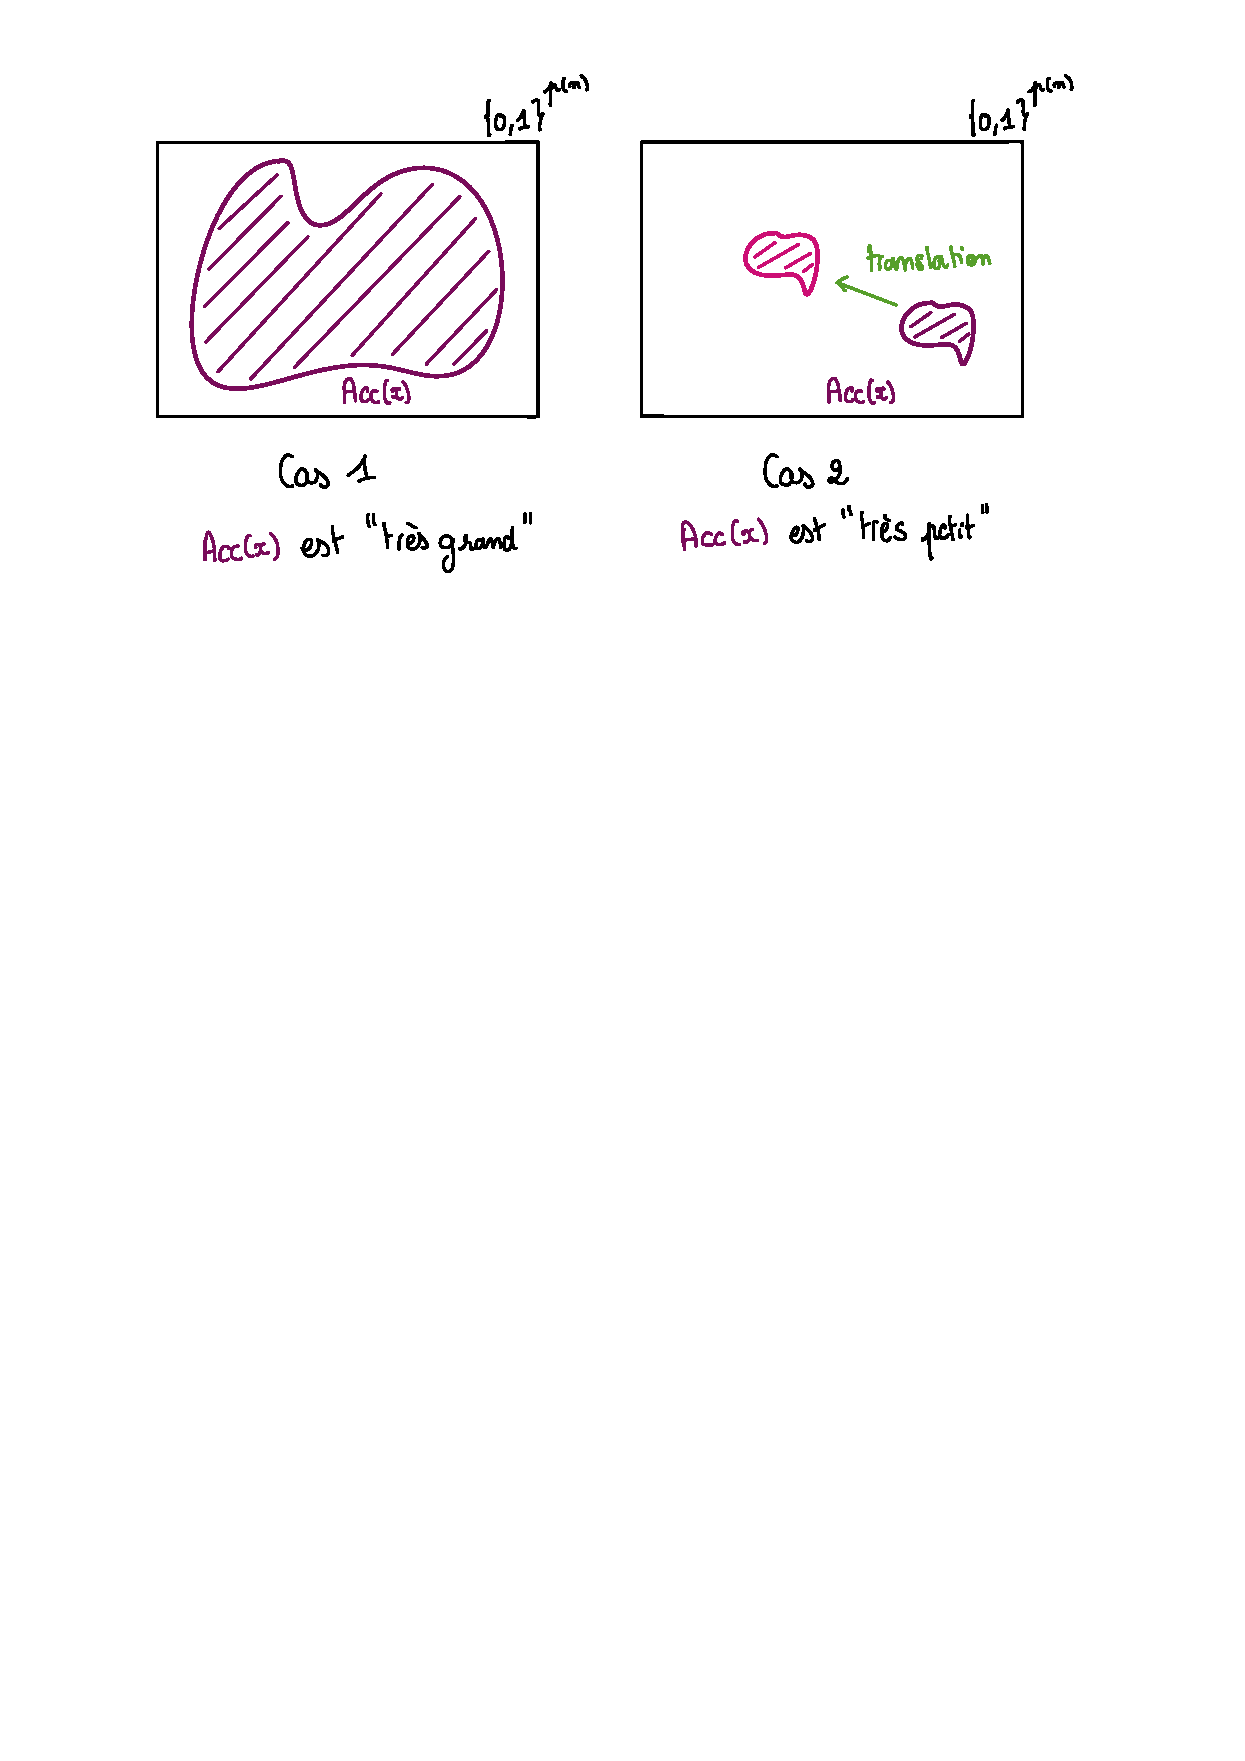
\includegraphics[width=0.85\textwidth,clip, trim=2cm 20cm 2.5cm 1cm]{figures/bpp_acc_ph.pdf}
      \caption{Les deux cas à distinguer}
    \end{figure}

    L'idée est qu'on essaie de couvrir $\{\texttt{0},\texttt{1}\}^{p(n)}$ par un petit nombre de translations de $\mathrm{Acc}(x)$, où la translation par $t \in \{\texttt{0},\texttt{1}\}^{p(n)}$
    \begin{align*}
      \{\texttt{0},\texttt{1}\}^{p(n)} &\longrightarrow \{\texttt{0},\texttt{1}\}^{p(n)} \\
      x &\longmapsto x \oplus t
    ,\end{align*}
    où $\oplus$ est le XOR bit à bit. 
    On pourra couvrir $\{\texttt{0},\texttt{1}\}^{p(n)}$ uniquement dans le cas 1.
    
    On va écrire 
    \begin{align*}
      (*) \quad\quad
      x \in A \iff \exists t_1 \ldots t_m &\in \{\texttt{0},\texttt{1}\}^{p(n)}\\
      &\forall z \in \{\texttt{0},\texttt{1}\}^{p(n)} \quad \bigvee_{i=1}^n \code{x, z \oplus t_i} \in B
    ,\end{align*}
    où les $t_1,\ldots,t_m$ représentent les $m$ vecteurs de translation.

    Si cette équivalence est vraie avec $m$ polynomial en $n$, on aura montré $A \in \phSigma 2$.
    En effet, pour un certain $x$, on a
    \[
      \code{x,  z \oplus t_i} \in B \iff z \oplus t_i \in \mathrm{Acc}(x) \iff  z \in \mathrm{Acc}(x) \oplus t_i
    ,\]
    où $\mathrm{Acc}(x) \oplus t_i$ est le translaté de $\mathrm{Acc}(x)$.
    La formule $(*)$ dit donc que les $m$ translations de $\mathrm{Acc}(x)$ recouvrent $\{\texttt{0},\texttt{1}\}^{p(n)}$.

    La suite sera vue la prochaine fois.
  \end{prv}
\end{document}
